\documentclass[10pt,openright,twoside,french]{book}

\input philippe2013
\input philippe2013_cours
\input philippe2013_sections
\input philippe2013_chapitre


\begin{document}
\setcounter{chapter}{1}
\renewcommand\PartProgramme{Géométrie}
\chapter[Coordonnées d'un point dans le plan]{Coordonnées d'un point\\ dans le plan}\label{ch_coordonnees}

\section{Repère orthonormé}

\begin{Defi}
    Un \ipt{repère orthonormé} du plan $(O,I,J)$ est défini de façon unique par la donnée de trois points non alignés $O$, $I$ et $J$ tels que :
    \begin{itemize}
        \item $(OI) \bot (OJ)$ ;
        \item $OI = OJ$.
    \end{itemize}
    Le point $O$ est appelé \ipt{origine du repère}.\par
    La droite graduée $(OI)$, orientée de $O$ vers $I$, est appelé \ipt{axe des abscisses} et la droite graduée $(OJ)$, orientée de $O$ vers $J$, est appelée \ipt{axe des ordonnées}.\par
    La longueur $OI$ définit l'unité de longueur sur l'axe des abscisses et la longueur $OJ$ définit l'unité de longueur sur l'axe des ordonnées.\par
    Par définition, les deux axes sont perpendiculaires et les unités de longueur sont identiques.
\end{Defi}

\begin{center}
%  \begin{tikzpicture}[x={(0.5cm,0cm)},y={(0.4cm,0.5cm)}]]
%        %\draw[line width=1pt,color=gray!25,dashed] (-4,-4) grid (4,4);
%        \foreach \x in {-4,-3,...,4} \draw[color=gray!25,line width=1pt,dashed] (\x,-4)--(\x,4);
%        \foreach \x in {-4,-3,...,4} \draw[color=gray!25,line width=1pt,dashed] (-4,\x)--(4,\x);
%        \draw[->,blue](-4,0)--(4,0);
%        \draw[->,blue](0,-4)--(0,4);
%        \draw (0,0) node[below] {\footnotesize $O$};
%        \draw (1,-0.2) node[below] {\footnotesize $I$}; \draw (1,0) node {|};
%        \draw (0,1) node[left] {\footnotesize $J$}; \draw (0,1) node {--};
%        \draw (0,-4) node[below] {Repère du plan};
%    \end{tikzpicture}\qquad%
%    \begin{tikzpicture}[x={(0.5cm,0cm)},y={(0cm,0.25cm)}]]
%        %\draw[line width=1pt,color=gray!25,dashed] (-4,-4) grid (4,4);
%        \foreach \x in {-4,-3,...,4} \draw[color=gray!25,line width=1pt,dashed] (\x,-4)--(\x,4);
%        \foreach \x in {-4,-3,...,4} \draw[color=gray!25,line width=1pt,dashed] (-4,\x)--(4,\x);
%        \draw[->,blue](-4,0)--(4,0);
%        \draw[->,blue](0,-4)--(0,4);
%        \draw (0,0) node[below left] {\footnotesize $O$};
%        \draw (1,-0.2) node[below] {\footnotesize $I$}; \draw (1,0) node {|};
%        \draw (0,1) node[left] {\footnotesize $J$}; \draw (0,1) node {--};
%        \draw (0,-4) node[below] {Repère orthogonal};
%    \end{tikzpicture}\par\medskip
    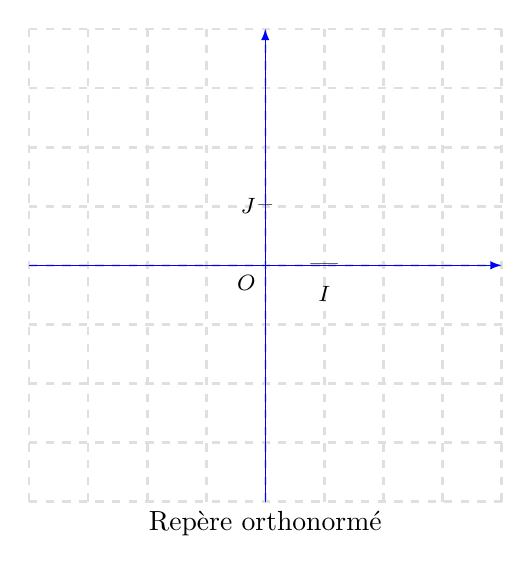
\begin{tikzpicture}[scale=0.75,>=latex]
        %\draw[line width=1pt,color=gray!25,dashed] (-4,-4) grid (4,4);
        \foreach \x in {-4,-3,...,4} \draw[color=gray!25,line width=1pt,dashed] (\x,-4)--(\x,4);
        \foreach \x in {-4,-3,...,4} \draw[color=gray!25,line width=1pt,dashed] (-4,\x)--(4,\x);
        \draw[->,blue](-4,0)--(4,0);
        \draw[->,blue](0,-4)--(0,4);
        \draw (0,0) node[below left] {\footnotesize $O$};
        \draw (1,-0.2) node[below] {\footnotesize $I$}; \draw (1,0) node {|};
        \draw (0,1) node[left] {\footnotesize $J$}; \draw (0,1) node {--};
        \draw (0,-4) node[below] {Repère orthonormé};
    \end{tikzpicture}
\end{center}

\section{Coordonnées d'un point}

On considère un point $M$ du plan dans un repère $(O,I,J)$ orthonormé.\par
On trace la parallèle à $(OJ)$ passant par $M$. Elle coupe l'axe des abscisses en $H$.\par
On trace la parallèle à $(OI)$ passant par $M$. Elle coupe l'axe des ordonnées en $K$.\medskip

\begin{Defi}
    \begin{enumerate}
        \item Sur l'axe $(OI)$, le nombre réel associé à $H$ est appelé \ipt{abscisse} du point $M$, que l'on note $x_M$.
        \item Sur l'axe $(OJ)$, le nombre réel associé à $K$ est appelé \ipt{ordonnée} du point $M$, que l'on note $y_M$.
        \item Le couple $(x_M \pv y_M)$ est alors appelé \ipt{coordonnées} du point $M$ et l'on note $M(x_M \pv y_M)$.
    \end{enumerate}
\end{Defi}\clearpage

\begin{Exemple}
\strut\par
\begin{minipage}{0.5\linewidth}
    Sur la figure ci-contre, l'abscisse de $M$ est égale à $3$ et son ordonnée est égale à $2,5$. On dira que les coordonnées de $M$ sont $(3 \pv 2,5)$ et on note $M(3 \pv 2,5)$.
\end{minipage}\quad
\begin{minipage}{0.4\linewidth}
\begin{center}
    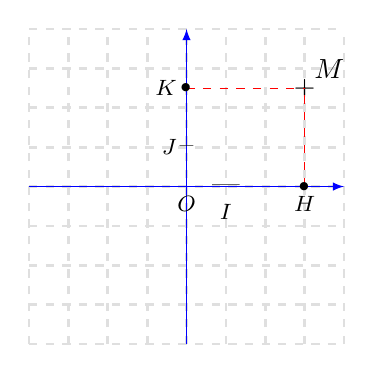
\begin{tikzpicture}[scale=0.5,>=latex]
        \foreach \x in {-4,-3,...,4} \draw[color=gray!25,line width=1pt,dashed] (\x,-4)--(\x,4);
        \foreach \x in {-4,-3,...,4} \draw[color=gray!25,line width=1pt,dashed] (-4,\x)--(4,\x);
        \draw[->,blue](-4,0)--(4,0);
        \draw[->,blue](0,-4)--(0,4);
        \draw (0,0) node[below] {\footnotesize $O$};
        \draw (1,-0.2) node[below] {\footnotesize $I$}; \draw (1,0) node {|};
        \draw (0,1) node[left] {\footnotesize $J$}; \draw (0,1) node {--};
        \draw (3,2.5) node[above right]{$M$}; \draw (3,2.5) node{$+$};
        \draw[dashed,red] (0,2.5)--(3,2.5); \draw (0,2.5) node[left]{\footnotesize$K$}; \draw (0,2.5) node{\rouge{$_\bullet$}};
        \draw[dashed,red] (3,0)--(3,2.5); \draw (3,0) node[below]{\footnotesize$H$}; \draw (3,0) node{\rouge{$_\bullet$}};
    \end{tikzpicture}
    \end{center}
\end{minipage}
\end{Exemple}

\begin{Rmq}
    Dans un  repère $(O,I,J)$, $A \in (OI) \Leftrightarrow y_A = 0$ et $B \in (OJ) \Leftrightarrow x_B = 0$.\par
    En particulier,  les coordonnées de l'origine du repère sont $(0 \pv 0)$, celle de $I$ sont $(1 \pv 0)$ et celle de $J$ sont $(0 \pv 1)$.\par
\end{Rmq}

\section{Distances dans un repère orthonormé}
On se place dans un repère \textbf{orthonormé} du plan $(O,I,J)$ et on considère deux points $A(x_A \pv y_A)$ et $B(x_B \pv y_B)$.\par\medskip

\begin{Prop}[(partiellement démontrée en exercice)]
    \begin{enumerate}
        \item Lorsque $x_A = x_B$, on pose $AB = y_B - y_A$ lorsque $y_B > y_A$ ou bien $AB = y_A - y_B$ lorsque $y_A > y_B$.
        \item Lorsque $y_A = y_B$, on pose $AB = x_B - x_A$ lorsque $x_B > x_A$ ou bien $AB = x_A - x_B$ lorsque $x_A > x_B$.
    \end{enumerate}
\end{Prop}\medskip

\begin{Rmq}
    Dans le premier cas, $(AB)$ est parallèle à l'axe des ordonnées et dans le second cas, $(AB)$ est parallèle à l'axe des abscisses.
\end{Rmq}\medskip

\begin{Exemple}
\strut

\begin{center}
\begin{tikzpicture}[>=latex]
        \draw[->,blue](-2.5,0)--(4,0);
        \draw[->,blue](0,-2)--(0,3.5);
        \draw (0,0) node[below left] {\footnotesize $O$};
        \draw (1,-0.1) node[below] {\footnotesize $I$}; \draw (1,0) node {|};
        \draw (0,1) node[left] {\footnotesize $J$}; \draw (0,1) node {--};
        \draw [dash pattern=on 5pt off 5pt] (-2,0)--(-2,2.5);
        \draw [dash pattern=on 5pt off 5pt] (1.5,0)-- (1.5,2.5);
        \draw [dash pattern=on 5pt off 5pt] (1,0.5)--(0,0.5);
        \draw [dash pattern=on 5pt off 5pt] (1,1.5)-- (0,1.5);
        \begin{scriptsize}
            \coordinate (A) at (-2,2.5); \draw (A) node[above left]{$A$}; \draw (-2,0) node[below] {$x_A$};
            \coordinate (B) at (1.5,2.5); \draw (B) node[above left]{$B$}; \draw (1.5,0) node[below] {$x_B$};
            \coordinate (C) at (1,1.5); \draw (C) node[right]{$C$}; \draw (0,1.5) node[left] {$y_C$};
            \coordinate (D) at (1,0.5); \draw (D) node[right]{$D$}; \draw (0,0.5) node[left]{$y_D$};
        \end{scriptsize}
        \draw (A) node {$\times$};\draw (B) node {$\times$};\draw (C) node {$\times$};\draw (D) node {$\times$};
        \draw[red] (A)--(B); \draw[red] (C)--(D);
        \draw (2.5,2) node[above right] {$AB = x_B - x_A$};
        \draw (2.5,2) node[below right] {$CD = y_C - y_D$};
\end{tikzpicture}
\end{center}
\end{Exemple}

\subsection{Calcul de distance}
\begin{Prop}
    La distance entre les points $A$ et $B$, autrement dit la longueur du segment $[AB]$, est égale à :
    \[AB = \sqrt{(x_B - x_A)^2 + (y_B - y_A)^2}\]
\end{Prop}\clearpage

\begin{Demo}
\begin{minipage}{0.55\linewidth}
On considère la figure ci-contre. Le point $C$ a pour coordonnées $(x_B \pv y_A)$ et, par conséquent, le triangle $ABC$ est rectangle en $C$.\par
D'après le théorème de Pythagore, on a \[AB^2 = AC^2 + BC^2.\]
Par construction, $A$ et $C$ ont la même ordonnée donc $AC^2 = (x_B - x_A)^2$. De même, puisque $B$ et $C$ ont la même abscisse, $BC^2 = (y_B - y_A)^2$.\par
Ainsi, $AB^2 = (x_B - x_A)^2 + (y_B - y_A)^2$ (qui est un nombre positif) donc finalement :
    \[AB = \sqrt{(x_B - x_A)^2 + (y_B - y_A)^2}\]
\end{minipage}\qquad
\begin{minipage}{0.4\linewidth}
\begin{center}
    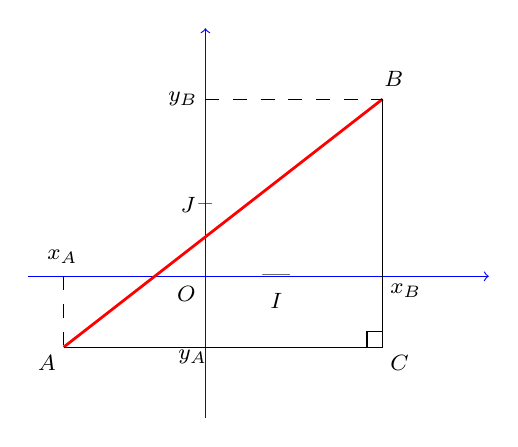
\begin{tikzpicture}[scale=0.9]
            \draw[->,blue](-2.5,0)--(4,0);
            \draw[->,blue](0,-2)--(0,3.5);
            \draw (0,0) node[below left] {\footnotesize $O$};
            \draw (1,-0.1) node[below] {\footnotesize $I$}; \draw (1,0) node {|};
            \draw (0,1) node[left] {\footnotesize $J$}; \draw (0,1) node {--};
            \draw (2.5,-0.78) -- (2.28,-0.78) -- (2.28,-1) -- (2.5,-1) -- cycle;
            \draw[line width=1pt,red] (-2,-1)-- (2.5,2.5);
            \draw (-2,-1)-- (2.5,-1);
            \draw (2.5,-1)-- (2.5,2.5);
            \draw [dash pattern=on 5pt off 5pt] (0,2.5)-- (2.5,2.5);
            \draw [dash pattern=on 5pt off 5pt] (-2,0)-- (-2,-1);
            \begin{scriptsize}
                \draw (-2,-1) node[below left] {\footnotesize$A$};
                \draw (2.66,2.78) node {\footnotesize$B$};
                \draw (2.5,-1) node[below right] {\footnotesize$C$};
                \draw (-0,2.5) node[left] {\footnotesize$y_B$};
                \draw (-2.02,0.28) node {\footnotesize$x_A$};
                \draw (-0.18,-1.14) node {\footnotesize$y_A$};
                \draw (2.5,0) node[below right] {\footnotesize$x_B$};
        \end{scriptsize}
    \end{tikzpicture}
\end{center}
\end{minipage}

\end{Demo}

\subsection{Milieu d'un segment}
\begin{Prop}
    On a appelle $P$ le milieu du segment $[AB]$. On a alors :
    \[x_P = \frac{x_A + x_B}{2} \qetq y_P = \frac{y_A + y_B}{2}.\]
\end{Prop}

\begin{Demo}
    \begin{minipage}{0.5\linewidth}
        \textbf{1\ier cas : $x_A = x_B$ ou $y_A = y_B$.}\par
        On suppose que $y_A = y_B$ et $x_B > x_A$. $P$ est le milieu de $[AB]$ si, et seulement si, $P \in [AB]$ et $PA = PB$.\par
        $P \in [AB] \Leftrightarrow y_P = y_A = y_B$ et on a bien $y_P = \frac{y_A + y_B}{2}$.\par
        $PA = PB \Leftrightarrow x_P - x_A = x_B - x_P \Leftrightarrow 2x_p = x_B + x_A$ et on a bien $x_P = \frac{x_A+ x_B}{2}$.
    \end{minipage}\quad
    \begin{minipage}{0.4\linewidth}
        \begin{center}
        \begin{tikzpicture}[scale=0.75]
                \begin{scriptsize}
                    \coordinate (A) at (0.5,2.5); \draw (A) node[above=5pt]{$A$};
                    \coordinate (C) at (0.5,0); \draw (C) node[below] {$x_A$};
                    \draw[dashed] (A)--(C);
                    \coordinate (B) at (5,2.5); \draw (B) node[above=5pt]{$B$};
                    \coordinate (D) at (5,0); \draw (D) node[below] {$x_B$};
                    \draw[dashed] (B)--(D);
                    \shorthandoff{!}
                    \coordinate (P) at ($ (A)!.5!(B) $); \draw (P) node {\rouge{$+$}} node[above=5pt] {$P$};
                    \coordinate(M) at ($(A)!.5!(P)$);\coordinate(N) at ($(A)!1.5!(P)$);
                    \shorthandon{!}
                    \coordinate (K) at (2.75,0); \draw (K) node {\rouge{$+$}} node[below=3pt] {$x_P$};
                \end{scriptsize}
                \draw (A) node {$+$};\draw (B) node {$+$};\draw (P) node {\rouge{$+$}};\draw (K) node {\rouge{$+$}};
                \draw[->,blue](-0.5,0)--(6,0);
                \draw[->,blue](0,-0.5)--(0,3.5);
                \draw (0,0) node[below left] {\footnotesize $O$};
                \draw[dashed] (0,2.5)--(B);
                \draw[dashed,red] (K)--(P);
                \draw (M) node{\violet{/\!\!/}};\draw (N) node{\violet{/\!\!/}};
        \end{tikzpicture}
        \end{center}
    \end{minipage}\bigskip

    \begin{minipage}{0.5\linewidth}
        \textbf{2\ieme cas : $x_A \neq x_B$ et $y_A \neq y_B$.}\par
        On note $C$ le point de coordonnées $(x_B \pv y_A)$ de façon à ce que le triangle $ABC$ soit rectangle en $C$. On appelle $K$ le milieu de $[AC]$ et $L$ celui de $[BC]$.\par
        On constate pour commencer que $(BC)$ est parallèle à l'axe des ordonnées car $x_B = x_C$ et que $(AC)$ est parallèle à l'axe des abscisses puisque $y_A = y_C$.
        Dans le triangle $ABC$, $P$ est le milieu de $[AB]$ et $K$ est celui de $[AC]$. D'après le théorème de la droite des milieux, on en déduit que $(PK)$ est parallèle à $(BC)$ et donc $(PK)$ est parallèle à $(OJ)$ donc $x_P = x_K = \frac{x_A + x_C}{2}$ donc $x_P = \frac{x_A + x_B}{2}$.\par
        En utilisant le point $L$, on obtiendrait de même $y_P = \frac{y_A + y_B}{2}$.
    \end{minipage}\quad
    \begin{minipage}{0.4\linewidth}
        \begin{center}
        \begin{tikzpicture}[scale=0.75]
                \begin{scriptsize}
                    \coordinate (A) at (0.5,1.5); \draw (A) node[above=5pt]{$A$};
                    \coordinate (C) at (0.5,0); \draw (C) node[below] {$x_A$};
                    \draw[dashed] (A)--(C);
                    \coordinate (B) at (5,3.5); \draw (B) node[above=5pt]{$B$};
                    \coordinate (D) at (5,0); \draw (D) node[below] {$x_B$};
                    \draw[dashed] (B)--(D);
                    \coordinate (Z) at (5,1.5);
                    \shorthandoff{!}
                    \coordinate (P) at ($ (A)!.5!(B) $); \draw (P) node {\rouge{$+$}} node[above=5pt] {$P$};
                    \coordinate(M) at ($(A)!.5!(P)$);\coordinate(N) at ($(A)!1.5!(P)$);
                    \coordinate(W) at ($(A)!.5!(Z)$);\coordinate(U) at ($(B)!.5!(Z)$);
                    \shorthandon{!}
                    \coordinate (K) at (2.75,0); \draw (K) node {\rouge{$+$}} node[below=5pt] {$x_P$};
                    \draw (Z) node[right]{$C$};
                    \draw (W) node[below right] {$K$};
                    \draw (U) node[right]{$L$};
                \end{scriptsize}
                \draw (A) node {$+$};\draw (B) node {$+$};\draw (P) node {\rouge{$+$}};\draw (K) node {\rouge{$+$}};
                \draw[->,blue](-0.5,0)--(6,0);
                \draw[->,blue](0,-0.5)--(0,3.5);
                \draw (0,0) node[below left] {\footnotesize $O$};
                \draw (A)--(B)--(Z)--cycle;
                \draw (M) node{\violet{$||$}};\draw (N) node{\violet{$||$}};
                \draw[red] (P)--(W); \draw[dashed,red] (K)--(W);
                \draw (U) node{$+$};
        \end{tikzpicture}
        \end{center}
    \end{minipage}
\end{Demo}

\section{Applications}
\begin{Exemple}[s]
On se place dans un repère orthonormé $(O,I,J)$ :
\begin{enumerate}
    \item Que peut-on dire du triangle $ABC$ tel que $A(-4 \pv 3)$, $B(-4\pv-5)$ et $C(3\pv-1)$ ?
    \item On considère le point $D$ de coordonnées $(x_D \pv y_D)$. On appelle $E$, son symétrique par rapport à $(OI)$ et $F$ son symétrique par rapport à $(OJ)$. Calculer les coordonnées de $E$ et $F$ en fonction de celles de $D$.
    \item On considère le point $G$ de coordonnées $(x_G \pv y_G)$ et on construit $H$, son symétrique par rapport à $O$. Calculer les coordonnées de $H$ en fonction de celles de $G$.
    \item On considère les quatre points suivants :
    \[K(-4\pv -1) \qq I(1 \pv 0) \qq L(2\pv2) \qetq M(-3\pv1).\]
    Démontrer de deux façons différentes que le quadrilatère $KILM$ est un parallélogramme.
\end{enumerate}
\end{Exemple}

\end{document}

